\documentclass[dvipdfmx]{jsarticle}
\usepackage[dvipdfmx]{graphicx}
\usepackage{amsmath, amssymb}
\usepackage{mathtools}
\usepackage{here}
\begin{document}
\title{週間進捗報告}
\author{権藤陸}
\date{5月25日}
\maketitle
\section{進捗}
\begin{itemize}
    \item いただいた論文の読み込み
    \item スライドの作成
\end{itemize}



\section{実装}

\begin{figure}[H]
\begin{center}
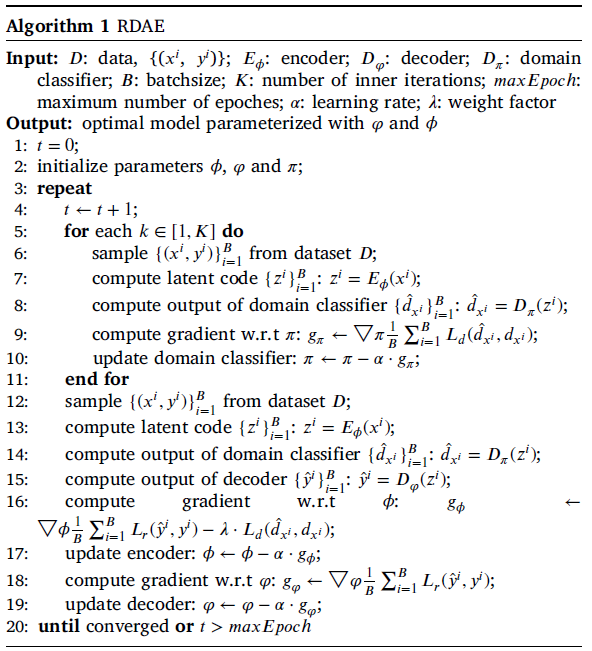
\includegraphics[width=0.6\linewidth]{./rdae_algorithm.png}
\end{center}
\caption{RDAEのアルゴリズム(擬似コード)}
\end{figure}
\begin{itemize}
    \item 勾配降下法によるパラメータの更新
    
パラメータは$\phi: エンコーダ$,$\varphi: デコーダ$,$\pi: ドメイン分類器$

    \item コードは近日中にgithubで公開と記述
    \item $\alpha$は初期値0.0005で550バッチごとに0.01ずつ減少
    \item $\lambda$は0.01
    \item \textit{maxEpoch}は100
\end{itemize}
\section{考察}
\underline{本研究におけるいくつかの制限}
\begin{itemize}
    \item データセットに偏りがある.具体的には,平均年齢と血圧が一般的な集団よりも高いICUの患者から得たデータである.
    \item データの各レコードあたりの時間が8~592秒で,確保されているサンプル数は32と少ないため,ドメインの学習には十分でない可能性がある.
    \item 用いたモデルは,ブラックボックス的なモデルであり,解釈可能性に欠ける.
    \item ドメイン分類器の損失を計算する際に,異なるドメインが互いに独立であるという仮定をしているため,ドメイン間の類似性は無視されている
    \item 本研究を含むほとんどの研究は,血圧波形予測を,記録中のサンプルが独立で時間的相関は考慮されていない状態で行っている.
\end{itemize}
\section{計画}
\begin{itemize}
    \item 関連研究の調査
    \item 発表スライドの作成
\end{itemize}


\end{document}